%% tp4.tex — Presentacion SdS TP4: dinamica molecular regida por el paso temporal
%%           (oscilador amortiguado + billar circular)
%%
%% Compilar desde presentaciones/tp4/:  latexmk -pdf tp4.tex   (o pdflatex dos veces)
%% Estilo: ../sdsbeamer.sty (por \input@path, sin symlink).
%% Figuras: ../../tp4-time-driven-md/analysis/figures/{ej1,ej2}/  y  figuras/ (locales: fotogramas)
%% Animaciones: fotograma + link (el PDF de entrega no lleva video embebido).
%% Entrega: SdS_TP4_2026Q2G02CS2_Presentación.pdf (campus, 23/10/2026 13 hs).
%%
%% Estructura (docs/GuiaPresentaciones.md §2 y ../AGENTS.md §5.3), 13 min:
%%   Introduccion (<1 min, 2 diap.: sistema real + modelo general) -> Implementacion (solo motor)
%%   -> Simulaciones (sistema particular, parametros, esquemas, observables, realizaciones y
%%   tiempos; sin resultados) -> Resultados -> Conclusiones (1 diap.) -> cierre -> uso de IA (2.5).
%% Resultados, por input (animacion -> evolucion temporal -> input vs observable):
%%   oscilador (sistema 1: una sola diapositiva, sin intro ni animacion, enunciado) ->
%%   paso temporal (2.1a) -> numero de particulas (2.1b y 2.4a: mismas corridas, mismo input) ->
%%   posicion de los obstaculos (2.2) -> distribucion de velocidades (2.3).
%% El sistema 1 va al principio de Resultados y no antes de la Introduccion: la presentacion
%%   arranca con la introduccion (../AGENTS.md §8.6) y el enunciado prohibe darle introduccion.
%% Resultados y numeros: ../../tp4-time-driven-md/AGENTS.md (seccion 6).
%%
%% Pendientes marcados con "% TODO:" (grep -n "TODO" tp4.tex).
% TODO: 34 diapositivas (TP3, también de 13 min, tenía 32): ensayar con las animaciones.
% TODO: ejes verticales solo con símbolo (<F_u>, F_u, <t_90>, f(v)): la guía los pide en
%   palabras. Paso: "Paso temporal (s)" en ecm_vs_dt y "Paso de integración (s)" en las del
%   billar; unificar.
% Figuras de analysis/figures sin usar: energia_costo_dt (corridas en paralelo, no es benchmark),
%   energia_esquemas_dt (ver TODO de Implementación), red_hexagonal (letra muy chica para una
%   diapositiva; la condición inicial va en texto), t90_vs_n, t100_vs_n, t90_vs_densidad y
%   t100_vs_densidad (reemplazadas por t90_t100_vs_densidad), fu_vs_t_xo_N{60,20,10} (alcanza
%   con una evolución típica), choques_{particulas,obstaculos}_vs_xo (ver TODO del 2.2),
%   ecm_dt4_vs_dt y ecm_vs_dt_tramo (solo análisis).

\documentclass[aspectratio=169]{beamer}
\makeatletter\def\input@path{{../}}\makeatother
\usepackage{sdsbeamer}
\usepackage{tikz}
\usetikzlibrary{arrows.meta,positioning,calc}
\microtypesetup{expansion=false}

\graphicspath{{../../tp4-time-driven-md/analysis/figures/}{figuras/}}

% Animacion: fotograma fijo representativo + enlace explicito debajo (GuiaPresentaciones 2.4.8).
% El valor de la variable va debajo del fotograma.
% \nolinkurl (no \texttt): los IDs pueden tener "_" y el texto se copia tal cual desde el PDF.
\newcommand{\yt}[1]{\href{https://youtu.be/#1}{\nolinkurl{youtu.be/#1}}}
% Fotograma de animacion de alto #1: figuras/#2 si existe; si no, un recuadro con el nombre
% esperado (cuadro de animate_billiard.py: 8.6 x 9.2, casi cuadrado). \IfFileExists no busca en
% \graphicspath: por eso la ruta explicita figuras/.
\newcommand{\fotograma}[2]{%
  \IfFileExists{figuras/#2}%
    {\includegraphics[height=#1]{figuras/#2}}%
    {\fcolorbox{black!35}{black!4}{\parbox[c][\dimexpr#1\relax][c]{\dimexpr#1*93/100\relax}{%
      \centering\color{black!55}\small Fotograma pendiente\par\vspace{0.3em}
      \scriptsize\texttt{\detokenize{#2}}\par}}}%
}
%   \animsola{<fotograma>}{<enlace>}
\newcommand{\animsola}[2]{%
  \centering
  \fotograma{0.70\textheight}{#1}\par\vspace{0.3em}
  {\large #2}\par
}
% Dos animaciones (valores extremos del input), cada una con su valor y su enlace.
%   \animdos{<fotograma 1>}{<valor 1>}{<enlace 1>}{<fotograma 2>}{<valor 2>}{<enlace 2>}
\newcommand{\animdos}[6]{%
  \begin{columns}[T]
    \begin{column}{0.48\textwidth}
      \centering\fotograma{0.62\textheight}{#1}\par\vspace{0.2em}
      #2\par\vspace{0.1em}{\small #3}\par
    \end{column}
    \begin{column}{0.48\textwidth}
      \centering\fotograma{0.62\textheight}{#4}\par\vspace{0.2em}
      #5\par\vspace{0.1em}{\small #6}\par
    \end{column}
  \end{columns}%
}
\newcommand{\kT}{k_{\mathrm{B}}T}

\title{Dinámica molecular regida por el paso temporal}
\subtitle{Simulación de Sistemas - ITBA}
\author[Grupo 2]{%
  Arancibia Nicolás -- Legajo 64481\\
  Morantes Agustín -- Legajo 61306\\
  Ronda Agustín -- Legajo 64507}
\institute[ITBA]{Grupo 2 --- Comisión S2 --- Instituto Tecnológico de Buenos Aires}
% TODO: confirmar la fecha de la presentación oral (la entrega del PDF es el 23/10/2026).
\date{23 de octubre de 2026}

\begin{document}

\begin{frame}[plain]
  \titlepage
\end{frame}

% ==========================================================================
\section{Introducción}
% Sistema real + ecuaciones del modelo general (sin sistema particular ni método de
% resolución). < 1 min, max 3 diapositivas.
% ==========================================================================

\begin{frame}{Billar circular}
  \begin{columns}[c]
    \begin{column}{0.54\textwidth}
      \begin{itemize}\setlength{\itemsep}{0.6em}
        \item Recinto circular cerrado por una pared fija, con dos obstáculos fijos.
        \item Partículas que chocan entre sí, con la pared y con los obstáculos.
        \item Toda partícula empieza \textcolor{blue}{fresca} y pasa a
          \textcolor{red}{usada} al tocar un obstáculo por primera vez; después sigue
          moviéndose e interactuando.
        \item Se estudia cuánto tardan en usarse según la posición de los obstáculos y la
          densidad.
      \end{itemize}
    \end{column}
    \begin{column}{0.44\textwidth}
      \centering
      % Esquema (no a escala): obstaculos negros, frescas azules, usadas rojas.
      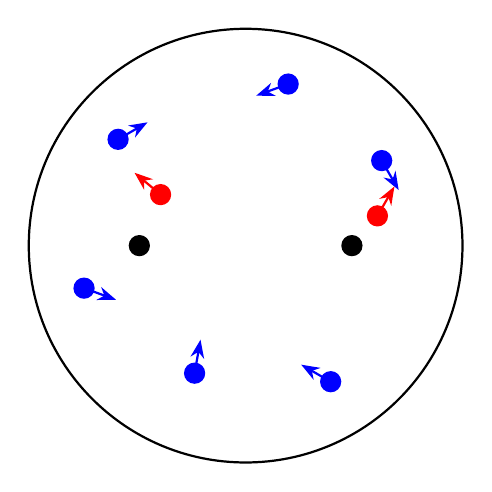
\begin{tikzpicture}[scale=5.4, >=Stealth]
        \draw[thick] (0,0) circle (0.51);
        \fill (-0.25,0) circle (0.025);
        \fill (0.25,0) circle (0.025);
        \foreach \x/\y/\a in {-0.3/0.25/30, 0.1/0.38/200, 0.32/0.2/-60, -0.12/-0.3/80,
                              0.2/-0.32/150, -0.38/-0.1/-20}
          {\fill[blue] (\x,\y) circle (0.025); \draw[->,blue,thick] (\x,\y) -- ++(\a:0.08);}
        \foreach \x/\y/\a in {0.31/0.07/60, -0.2/0.12/140}
          {\fill[red] (\x,\y) circle (0.025); \draw[->,red,thick] (\x,\y) -- ++(\a:0.08);}
      \end{tikzpicture}
    \end{column}
  \end{columns}
\end{frame}

\begin{frame}{Modelo}
  \begin{columns}[c]
    \begin{column}{0.54\textwidth}
      \small
      \begin{itemize}\setlength{\itemsep}{0.4em}
        \item $m\,\ddot{\vect{r}}_i = \vect{F}_i$; resortes normales, sin fricción ni disipación:
          \[
            \vect{F}_i = \sum_{j\,:\,\xi_{ij} > 0} -k\,\xi_{ij}\,\hat{\vect{e}}_{ij}
          \]
          \[
            \xi_{ij} = r_i + r_j - |\vect{r}_j - \vect{r}_i|, \qquad
            \hat{\vect{e}}_{ij} = \frac{\vect{r}_j - \vect{r}_i}{|\vect{r}_j - \vect{r}_i|}
          \]
        \item $j$: otras partículas, obstáculos fijos o la imagen de la pared.
        \item Pared de radio $R$, normal $\hat{\vect{n}} = \vect{r}_i/|\vect{r}_i|$: imagen fija
          del otro lado del contacto $C$:
          \[
            \vect{r}_{\mathrm{img}} = (R + r_i)\,\hat{\vect{n}}, \qquad
            \xi_{iw} = |\vect{r}_i| + r_i - R
          \]
      \end{itemize}
    \end{column}
    \begin{column}{0.44\textwidth}
      \centering
      % Particula i superpuesta con otra particula j (izquierda) y con la pared (derecha); la
      % imagen punteada esta del otro lado de C. No a escala. Centro de la pared a la izquierda,
      % fuera de la figura: el arco arranca en ($(-3.5,0)+(-24:4)$) para no meter (-3.5,0) en el
      % bounding box.
      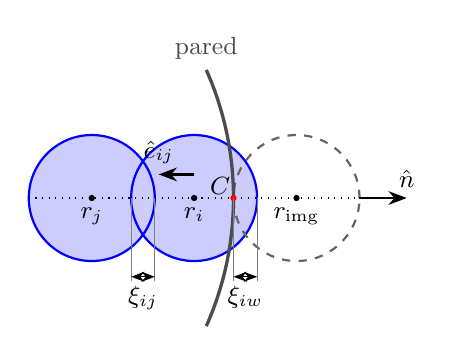
\begin{tikzpicture}[scale=1.0, >=Stealth]
        \fill[blue!20] (-1.3,0) circle (0.8);
        \fill[blue!20] (0,0) circle (0.8);
        \draw[blue, thick] (-1.3,0) circle (0.8);
        \draw[blue, thick] (0,0) circle (0.8);
        \draw[black!60, dashed, thick] (1.3,0) circle (0.8);
        \draw[very thick, black!70] ($(-3.5,0)+(-24:4)$) arc[start angle=-24, end angle=24, radius=4]
          node[above, font=\small] {pared};
        \draw[dotted] (-2.1,0) -- (2.1,0);
        \draw[->, thick] (2.1,0) -- (2.7,0) node[above, font=\small] {$\hat{\vect{n}}$};
        \draw[->, thick] (0,0.3) -- (-0.45,0.3) node[above, font=\small] {$\hat{\vect{e}}_{ij}$};
        \fill (-1.3,0) circle (0.04) node[below, font=\small] {$\vect{r}_j$};
        \fill (0,0) circle (0.04) node[below, font=\small] {$\vect{r}_i$};
        \fill (1.3,0) circle (0.04) node[below, font=\small] {$\vect{r}_{\mathrm{img}}$};
        \fill[red] (0.5,0) circle (0.04);
        \node[above left, inner sep=1pt, font=\small] at (0.5,0) {$C$};
        \draw[thin, black!50] (-0.8,0) -- (-0.8,-1.05);
        \draw[thin, black!50] (-0.5,0) -- (-0.5,-1.05);
        \draw[<->] (-0.8,-1.0) -- (-0.5,-1.0) node[midway, below, font=\small] {$\xi_{ij}$};
        \draw[thin, black!50] (0.5,0) -- (0.5,-1.05);
        \draw[thin, black!50] (0.8,0) -- (0.8,-1.05);
        \draw[<->] (0.5,-1.0) -- (0.8,-1.0) node[midway, below, font=\small] {$\xi_{iw}$};
      \end{tikzpicture}
    \end{column}
  \end{columns}
\end{frame}

% ==========================================================================
\section{Implementación}
% Solo el motor. Sin post-proceso ni formatos de I/O.
% ==========================================================================

% Lazo de BilliardRun / VelocityVerlet / ContactForces (md-java). Velocity Verlet en la forma
% "medio paso de velocidad, posición, fuerzas, medio paso de velocidad", equivalente a las
% ecuaciones de la teórica que van debajo.
% TODO: el enunciado dice "esquema de Verlet" y todo el sistema 2 se corrió con Velocity Verlet
%   (decisión abierta 1 de tp4-time-driven-md/AGENTS.md). Decidir cómo se justifica: si hace
%   falta mostrarlo, energia_esquemas_dt.png (mismo <ε> que Verlet original en todo el rango)
%   suma una diapositiva en Resultados.
\begin{frame}{Motor: lazo de paso temporal}
  \centering
  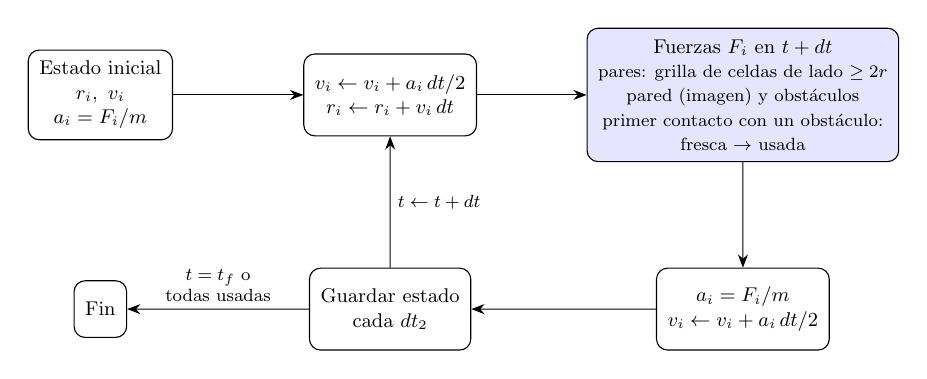
\begin{tikzpicture}[>=Stealth, font=\small, scale=0.8, every node/.append style={scale=0.8},
      caja/.style={draw, rounded corners, align=center, inner sep=5pt, minimum height=1.3cm},
      clave/.style={caja, fill=blue!10}]
    \node[caja]  (ini)  at (0, 0)      {Estado inicial\\ $\vect{r}_i,\ \vect{v}_i$\\
                                        $\vect{a}_i = \vect{F}_i/m$};
    \node[caja]  (med)  at (4.6, 0)    {$\vect{v}_i \leftarrow \vect{v}_i + \vect{a}_i\,dt/2$\\
                                        $\vect{r}_i \leftarrow \vect{r}_i + \vect{v}_i\,dt$};
    \node[clave] (fza)  at (10.2, 0)   {Fuerzas $\vect{F}_i$ en $t + dt$\\
                                        {\footnotesize pares: grilla de celdas de lado $\ge 2r$}\\
                                        {\footnotesize pared (imagen) y obstáculos}\\
                                        {\footnotesize primer contacto con un obstáculo:}\\
                                        {\footnotesize fresca $\to$ usada}};
    \node[caja]  (vel)  at (10.2, -3.4) {$\vect{a}_i = \vect{F}_i/m$\\
                                        $\vect{v}_i \leftarrow \vect{v}_i + \vect{a}_i\,dt/2$};
    \node[caja]  (save) at (4.6, -3.4)  {Guardar estado\\ cada $dt_2$};
    \node[caja, minimum height=0.9cm] (fin) at (0, -3.4) {Fin};
    \draw[->] (ini) -- (med);
    \draw[->] (med) -- (fza);
    \draw[->] (fza) -- (vel);
    \draw[->] (vel) -- (save);
    \draw[->] (save) -- node[right, font=\footnotesize] {$t \leftarrow t + dt$} (med);
    \draw[->] (save) -- node[above, font=\footnotesize, align=center] {$t = t_f$ o\\ todas usadas} (fin);
  \end{tikzpicture}

  \vspace{0.2em}
  \begin{columns}[c]
    \begin{column}{0.22\textwidth}\raggedleft\small Velocity Verlet:\end{column}
    \begin{column}{0.70\textwidth}\small
      \vspace{-0.6em}
      \begin{align*}
        \vect{r}_i(t + dt) &= \vect{r}_i(t) + \vect{v}_i(t)\,dt + \tfrac{1}{2}\,\vect{a}_i(t)\,dt^2\\
        \vect{v}_i(t + dt) &= \vect{v}_i(t)
          + \tfrac{1}{2}\bigl[\vect{a}_i(t) + \vect{a}_i(t + dt)\bigr]\,dt
      \end{align*}
    \end{column}
  \end{columns}
\end{frame}

% ==========================================================================
\section{Simulaciones}
% Sistema particular, parametros fijos y variables, esquemas, observables, repeticiones y
% tiempos. Sin resultados: ni el inicio del estacionario ni la justificacion del dt (van en
% Resultados).
% ==========================================================================

% Sistema 2: parámetros fijos y variables, genéricos (no por estudio). El valor que toma cada
% parámetro en cada estudio va al costado de las figuras de Resultados. El sistema 1 no va acá:
% el enunciado limita el oscilador a una sola diapositiva, en Resultados.
\begin{frame}{Sistema}
  \begin{columns}[c]
    \begin{column}{0.46\textwidth}
      \centering
      % Esquema con las magnitudes (radios exagerados para que se vean).
      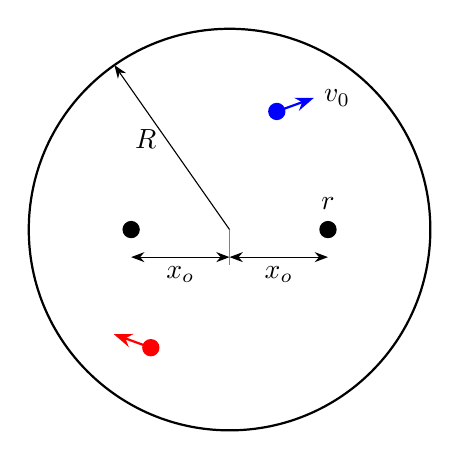
\begin{tikzpicture}[scale=5.0, >=Stealth]
        \draw[thick] (0,0) circle (0.51);
        \draw[->] (0,0) -- (125:0.51) node[pos=0.55, left] {$R$};
        \fill (-0.25,0) circle (0.022);
        \fill (0.25,0) circle (0.022);
        \node[above] at (0.25,0.025) {$r$};
        \draw[thin, black!50] (0,0) -- (0,-0.09);
        \draw[<->] (0,-0.07) -- (0.25,-0.07) node[midway, below] {$x_o$};
        \draw[<->] (-0.25,-0.07) -- (0,-0.07) node[midway, below] {$x_o$};
        \fill[blue] (0.12,0.3) circle (0.022);
        \draw[->,blue,thick] (0.12,0.3) -- ++(20:0.1) node[right, black] {$v_0$};
        \fill[red] (-0.2,-0.3) circle (0.022);
        \draw[->,red,thick] (-0.2,-0.3) -- ++(160:0.1);
      \end{tikzpicture}
    \end{column}
    \begin{column}{0.52\textwidth}
      \textbf{Parámetros fijos}
      \begin{itemize}\setlength{\itemsep}{2pt}
        \item $R = 0.51\uni{m}$, $r = 0.0175\uni{m}$
        \item $m = 0.025\uni{kg}$, $k = 10^{4}\uni{N/m}$
        \item $v_0 = 1\uni{m/s}$
      \end{itemize}
      \vspace{0.8em}
      \textbf{Parámetros variables}
      \begin{itemize}\setlength{\itemsep}{2pt}
        \item $dt$: $10^{-6}$ a $5\ten{-3}\uni{s}$
        \item $N$: 25 a 675
        \item $x_o$: $r$ a $R - r$, o sin obstáculos
      \end{itemize}
      \vspace{1.2em}
      {\small 10 realizaciones por configuración}
    \end{column}
  \end{columns}
\end{frame}

\begin{frame}{Observables: energía, costo y partículas usadas}
  \small
  \begin{columns}[T]
    \begin{column}{0.50\textwidth}
      \begin{itemize}\setlength{\itemsep}{0.6em}
        \item Energía total (contactos: pares, pared y obstáculos):
          \[
            E(t) = \sum_{i=1}^{N} \tfrac{1}{2}\,m\,|\vect{v}_i(t)|^2
              + \sum_{\text{contactos}} \tfrac{1}{2}\,k\,\xi^2
          \]
        \item Error medio de la energía, sobre los $K = 200$ estados guardados con $t_\ell > 0$:
          \[
            \varepsilon = \frac{1}{K}\sum_{\ell=1}^{K} \left|\frac{E(t_\ell) - E(0)}{E(0)}\right|
          \]
        \item Tiempo de ejecución: duración del lazo de integración.
      \end{itemize}
    \end{column}
    \begin{column}{0.48\textwidth}
      \begin{itemize}\setlength{\itemsep}{0.6em}
        \item $N_u(t)$: cantidad acumulada de partículas usadas; $F_u(t) = N_u(t)/N$.
        \item $t_{90} = \min\{t : F_u(t) \ge 0.9\}$\\[0.2em]
          $t_{100} = \min\{t : F_u(t) = 1\}$
        \item $\langle\varepsilon\rangle$, tiempo de ejecución, $\langle t_{90}\rangle$ y
          $\langle t_{100}\rangle$: promedio $\pm$ desvío estándar entre realizaciones.
        \item $\langle t_{90}\rangle$, $\langle t_{100}\rangle$ solo si llegan todas; si no, se
          informa $F_u(t_{\mathrm{max}})$.
      \end{itemize}
    \end{column}
  \end{columns}
\end{frame}

\begin{frame}{Observables: distribución de velocidades}
  \begin{itemize}\setlength{\itemsep}{0.55em}
    \item Rapidez $v_i = |\vect{v}_i|$; bins de ancho $\Delta v$ centrados en $v_b$;
      $N_b(t)$: partículas con $v_i$ en el bin $b$.
      \[
        f(v_b, t) = \frac{N_b(t)}{N\,\Delta v}, \qquad
        \bar{v}(t) = \frac{1}{N}\sum_{i=1}^{N} v_i(t)
      \]
    \item $\bar{v}(t)$ marca a ojo el inicio del estacionario, $t_{\mathrm{est}}$.
    \item $f(v)$ estacionaria: promedio de $f(v_b, t_\ell)$ sobre todos los estados con
      $t_\ell \ge t_{\mathrm{est}}$ de todas las realizaciones; barra: desvío de esos valores.
    \item Ajuste de Maxwell-Boltzmann en 2D, con $\kT$ como único parámetro:
      \[
        f_{\mathrm{MB}}(v) = \frac{m\,v}{\kT}\,\exp\!\left(-\frac{m\,v^2}{2\,\kT}\right), \qquad
        \mathcal{E}(\kT) = \sum_b \bigl[f(v_b) - f_{\mathrm{MB}}(v_b)\bigr]^2
      \]
  \end{itemize}
\end{frame}

% ==========================================================================
\section{Resultados}
% Por input: animacion -> evolucion temporal -> input vs observable.
% TODO: todos los fotogramas (figuras/anim_*.png) y links de YouTube están pendientes. Las
%   corridas largas de output/billiard/ no están en esta copia del repo.
% ==========================================================================

% --- Sistema 1 ------------------------------------------------------------
% Enunciado: UNA sola diapositiva, con la figura de ECM vs dt de los 4 métodos; sin
% introducción, ni animaciones, ni ninguna otra información: solo la figura, sin nada al costado.
% Leyenda de menor a mayor ECM. "¿Cuál es mejor?" (Beeman) va en Conclusiones.
% TODO: el ECM se calcula sobre los estados guardados cada 10^-2 s y no sobre todos los pasos
%   (letra del enunciado), y ya no se declara en la diapositiva: decidir si se recalcula.
\begin{frame}{Oscilador: error cuadrático medio vs paso temporal}
  \centering
  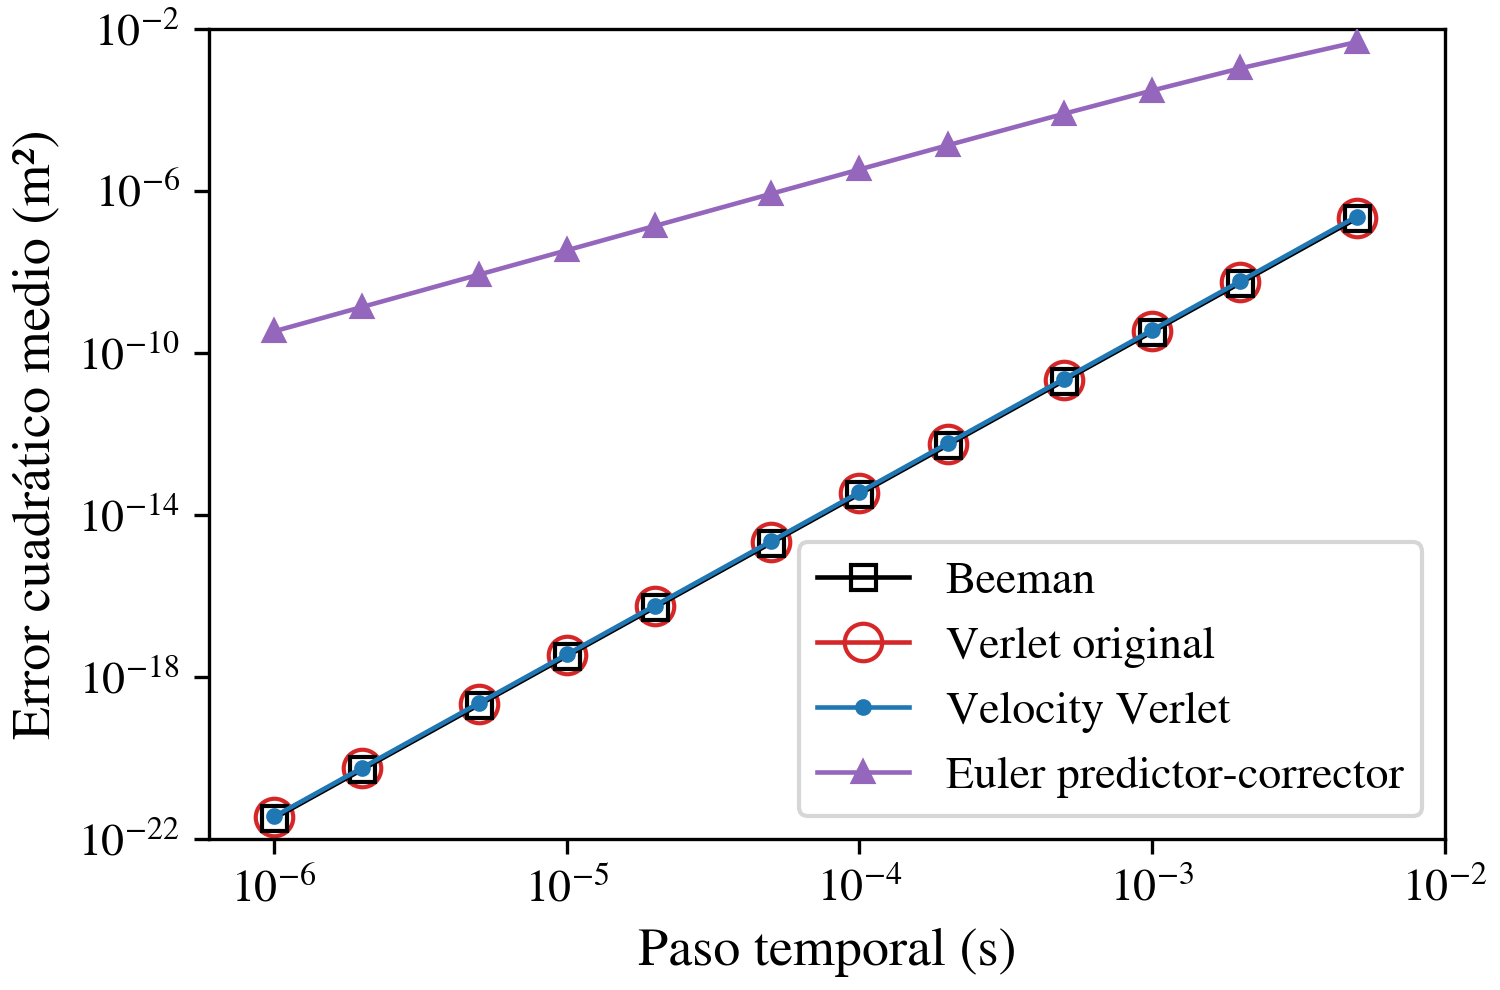
\includegraphics[width=\linewidth,height=0.82\textheight,keepaspectratio]{ej1/ecm_vs_dt.png}
\end{frame}

% --- Paso temporal (2.1a) ---------------------------------------------------

% TODO: elegir los dt de la animación. Propuesta: 10^-3 s (diverge) y 10^-5 s (elegido); las
%   corridas de output/billiard/energy_dt/ guardan cada 5e-2 s (200 cuadros en 10 s).
\begin{frame}{Paso temporal: animaciones con $N = 300$}
  \animdos{anim_energia_dt1e-3.png}{$dt = 10^{-3}\uni{s}$}{\yt{PENDIENTE}}
          {anim_energia_dt1e-5.png}{$dt = 10^{-5}\uni{s}$}{\yt{PENDIENTE}}
\end{frame}

\begin{frame}{Paso temporal: energía total vs tiempo}
  \figuraparam{ej2/energia_vs_t.png}{%
    $N = 300$, sin obstáculos, $t_f = 10\uni{s}$\\
    Una realización\\[0.5em]
    $dt \ge 10^{-3}\uni{s}$: la energía diverge (fuera de la figura)
  }
\end{frame}

% TODO: ¿mencionar la pendiente log-log 2.03 de <ε> vs dt (orden 2)? Si se afirma, mostrar el
%   ajuste.
\begin{frame}{Paso temporal: error medio de la energía vs paso}
  \figuraparam{ej2/energia_error_medio_dt.png}{%
    $N = 300$, sin obstáculos, $t_f = 10\uni{s}$\\
    10 realizaciones por punto\\[0.5em]
    $dt \ge 10^{-3}\uni{s}$: $\langle\varepsilon\rangle \ge 1$ (fuera de la figura)\\[0.5em]
    Elegido: $dt = 10^{-5}\uni{s}$, mayor potencia de 10 con
    $\langle\varepsilon\rangle < 10^{-4}$:\\
    $\langle\varepsilon\rangle = (5 \pm 2)\ten{-6}$
  }
\end{frame}

% --- Número de partículas (2.1b y 2.4a: mismas corridas) -----------------------

% TODO: animaciones de los extremos (decidido: N = 600 como alto, N = 25 propuesto como bajo),
%   re-corriendo una semilla ~20 s con estado fino. Existe larga_N600_s1.mp4 (estado cada 5 s).
%   ¿N = 675 en lugar de 600? Mostraría el anillo de usadas que traba el sistema (ver TODO de
%   Conclusiones).
\begin{frame}{Número de partículas: animaciones con $x_o = r$}
  \animdos{anim_densidad_N25.png}{$N = 25$}{\yt{PENDIENTE}}
          {anim_densidad_N600.png}{$N = 600$}{\yt{PENDIENTE}}
\end{frame}

% TODO: discutir el escalamiento (exponente local: paso temporal 0.15 -> 2, eventos 2.6 -> 13,
%   AGENTS.md §6). Si se dice, mostrarlo.
\begin{frame}{Número de partículas: tiempo de ejecución}
  \figuraparam{ej2/tiempo_vs_n.png}{%
    Obstáculos en contacto ($x_o = r$)\\
    $t_f = 30\uni{s}$, $dt = 10^{-5}\uni{s}$\\
    10 realizaciones por $N$\\[0.5em]
    Eventos: punto 1.1 del TP3 (mesa rectangular vacía, red hexagonal), misma computadora\\[0.5em]
    Paso temporal: desvío de 0.1 a 2.8\,\%, tapado por el símbolo
  }
\end{frame}

\begin{frame}{Número de partículas: fracción de usadas vs tiempo}
  \figuraparam{ej2/fu_vs_t_densidad.png}{%
    Obstáculos en contacto ($x_o = r$)\\
    10 realizaciones ($N = 675$: 1)\\
    Banda: desvío entre realizaciones\\[0.5em]
    $\rho = 31$, $367$, $734$ y $826\uni{m^{-2}}$
  }
\end{frame}

\begin{frame}{Número de partículas: realizaciones que no llegan a $F_u = 1$}
  \figuraparam{ej2/fu_vs_t_incompletas.png}{%
    Obstáculos en contacto ($x_o = r$)\\
    Una curva por realización\\[0.5em]
    $F_u(1500\uni{s})$:\\
    $N = 600$: 0.993 a 1.000 (10)\\
    $N = 625$: 0.92 a 0.95 (10)\\
    $N = 650$: 0.11 (1)\\
    $N = 675$: 0.01 (1)
  }
\end{frame}

\begin{frame}{Número de partículas: $\langle t_{90} \rangle$ y $\langle t_{100} \rangle$ vs densidad}
  \figuraparam{ej2/t90_t100_vs_densidad.png}{%
    Obstáculos en contacto ($x_o = r$)\\
    10 realizaciones por punto\\
    Solo los $N$ en que llegan las 10\\[0.5em]
    Mínimo en $\rho = 61\uni{m^{-2}}$ ($N = 50$):\\
    $\langle t_{90} \rangle = 23 \pm 4\uni{s}$\\
    $\langle t_{100} \rangle = 40 \pm 10\uni{s}$
  }
\end{frame}

% --- Posición de los obstáculos (2.2) ----------------------------------------

% TODO: elegir los x_o de la animación (propuesta: 0.25 m y R - r, el mejor y el peor de
%   fu_vs_t_xo_N100.png; o los extremos r y R - r).
\begin{frame}{Posición de los obstáculos: animaciones con $N = 100$}
  \animdos{anim_xo025_N100.png}{$x_o = 0.25\uni{m}$}{\yt{PENDIENTE}}
          {anim_xoborde_N100.png}{$x_o = R - r$}{\yt{PENDIENTE}}
\end{frame}

% TODO (figura): agregar una recta horizontal en F_u = 0.9 para cerrar la evolución con t_90.
\begin{frame}{Posición de los obstáculos: fracción de usadas vs tiempo}
  \figuraparam{ej2/fu_vs_t_xo_N100.png}{%
    $N = 100$\\
    10 realizaciones\\
    Banda: desvío entre realizaciones\\[0.5em]
    $R - r = 0.4925\uni{m}$
  }
\end{frame}

% TODO: el enunciado pide discutir si el x_o óptimo depende de la frecuencia de choques entre
%   partículas. Esta figura compara densidades; la frecuencia de choques está medida en
%   choques_particulas_vs_xo.png (12.8 y 2.15 s^-1 para N = 100 y 20), todavía sin decidir si va
%   (sumaría una diapositiva).
% TODO: avisar outliers de N = 20: x_o = 0.05 (21 ± 7 s, máx 33.6) y R - r (25 ± 8 s, máx 42.9).
\begin{frame}{Posición de los obstáculos: $\langle t_{90} \rangle$ vs posición}
  \figuraparam{ej2/t90_vs_xo.png}{%
    10 realizaciones por punto\\[0.5em]
    Todas llegan a $F_u = 0.9$ antes de $t_{\mathrm{max}} = 100\uni{s}$
  }
\end{frame}

% --- Distribución de velocidades (2.3) -----------------------------------------

% TODO: animación (¿partículas coloreadas por rapidez?). Sin corrida de animación todavía.
\begin{frame}{Distribución de velocidades: animación con $N = 100$}
  \animsola{anim_velocidades_N100.png}{\yt{PENDIENTE}}
\end{frame}

\begin{frame}{Distribución de velocidades: rapidez media vs tiempo}
  \figuraparam{ej2/rapidez_media_vs_t.png}{%
    $N = 100$, sin obstáculos, $t_f = 20\uni{s}$\\
    10 realizaciones\\
    Banda: desvío entre realizaciones\\[0.5em]
    Recta: inicio del estacionario, $t_{\mathrm{est}} = 1\uni{s}$\\[0.5em]
    $\bar{v} = 0.880 \pm 0.015\uni{m/s}$ ($t \ge t_{\mathrm{est}}$)
  }
\end{frame}

\begin{frame}{Distribución de velocidades: evolución de $f(v)$}
  \figuraparam{ej2/fv_evolucion.png}{%
    $N = 100$, sin obstáculos\\
    10 realizaciones\\
    $\Delta v = 0.1\uni{m/s}$\\
    Barra: desvío entre realizaciones\\[0.5em]
    $t = 0$: todas con $v_i = v_0 = 1\uni{m/s}$
  }
\end{frame}

% TODO: k_BT* no tiene incerteza calculada; revisar cuántas cifras se informan (12.41 mJ).
\begin{frame}{Distribución de velocidades: ajuste de $\kT$}
  \figuraparam{ej2/error_ajuste_mb.png}{%
    $\mathcal{E}(\kT) = \sum_b \bigl[f(v_b) - f_{\mathrm{MB}}(v_b)\bigr]^2$\\[0.5em]
    Recta: mínimo,\\ $\kT^{*} = 12.41\uni{mJ}$
  }
\end{frame}

% La diferencia entre m<v^2>/2 y m v0^2/2 sería energía guardada en los resortes: es una
% inferencia (no se midió E_p en estas corridas), no va a la diapositiva sin medirla.
\begin{frame}{Distribución de velocidades: $f(v)$ estacionaria}
  \figuraparam{ej2/fv_estacionaria_mb.png}{%
    $t \ge t_{\mathrm{est}} = 1\uni{s}$, 10 realizaciones\\
    $\Delta v = 0.05\uni{m/s}$\\
    Barra: desvío de los $f$ instantáneos\\[0.5em]
    $\kT^{*} = 12.41\uni{mJ}$\\
    $m\langle v^2 \rangle/2 = 12.32\uni{mJ}$\\
    $m v_0^2/2 = 12.50\uni{mJ}$
  }
\end{frame}

% 2.4b (opcional, mapa de calor de <t_90> en (x_o, N)): no hecho.

% ==========================================================================
\section{Conclusiones}
% Solo lo que está en las figuras de Resultados. Cuantificar.
% ==========================================================================

% TODO: el enunciado pregunta "¿por qué?" hay una densidad óptima. Las animaciones de N = 650 y
%   675 muestran un anillo de usadas que no se mueve alrededor de los obstáculos (AGENTS.md §6):
%   si se usa como explicación, tiene que estar mostrado en Resultados.
% Beeman: C = ECM/dt^4 = 330 contra 348 (Verlet original) y 364 (Velocity Verlet) m^2 s^-4, en
%   todo el rango de dt y en cada ventana de 1 s de t (tp4-time-driven-md/AGENTS.md §6).
\begin{frame}{Conclusiones}
  \small
  \begin{itemize}\setlength{\itemsep}{0.5em}
    \item Oscilador: Beeman da el menor ECM, por poco, en todo el rango de $dt$; Beeman,
      Verlet original y Velocity Verlet, de $10^{4}$ a $10^{12}$ veces menor que Euler
      predictor-corrector.
    \item Con $dt = 10^{-5}\uni{s}$ la energía se conserva con
      $\langle\varepsilon\rangle = (5 \pm 2)\ten{-6}$; con $dt \ge 10^{-3}\uni{s}$ diverge.
    \item Costo: eventos es más rápido hasta $N = 400$ y paso temporal desde $N = 500$
      ($100\uni{s}$ contra $850\uni{s}$ en $N = 675$).
    \item Densidad: $\langle t_{90} \rangle$ mínimo, $23 \pm 4\uni{s}$, en
      $\rho = 61\uni{m^{-2}}$; $1270 \pm 70\uni{s}$ en $\rho = 765\uni{m^{-2}}$; desde
      $\rho = 795\uni{m^{-2}}$ no llega a $F_u = 0.9$ en $1500\uni{s}$.
    \item Obstáculos ($N = 100$): $\langle t_{90} \rangle \approx 15\uni{s}$ con $x_o$ entre
      $0.15$ y $0.35\uni{m}$, contra $23 \pm 3\uni{s}$ en $x_o = r$ y $32 \pm 5\uni{s}$ en
      $x_o = R - r$; la misma meseta con $N = 60$ y $20$.
    \item Velocidades: estacionario desde $t = 1\uni{s}$; Maxwell-Boltzmann con
      $\kT^{*} = 12.41\uni{mJ}$, 0.7\,\% debajo de $m v_0^2/2$.
  \end{itemize}
\end{frame}

\begin{frame}[plain]
  \centering
  \vfill
  {\Huge Muchas gracias}
  \vfill
\end{frame}

% Punto 2.5 del enunciado: diapositiva extra, al final de la presentación oral.
% TODO (grupo): completar agente, modelo y forma de uso.
\begin{frame}{Uso de agentes de IA}
  \begin{itemize}\setlength{\itemsep}{1em}
    \item Agente: \textcolor{black!50}{[completar]}
    \item Modelo: \textcolor{black!50}{[completar]}
    \item Uso: \textcolor{black!50}{[completar]}
  \end{itemize}
\end{frame}

\end{document}
